\documentclass[journal,a4paper,twoside]{sty/IEEEtran}

\usepackage[utf8]{inputenc}
\usepackage[T1]{fontenc}
\usepackage[slovene]{babel}
\usepackage{sty/EVrevija}

\ifCLASSINFOpdf
   \usepackage[pdftex]{graphicx}
\else
   \usepackage[dvips]{graphicx}
\fi
\usepackage{epstopdf}
\usepackage{amsmath}

\begin{document}

\title{Avtomatska analiza testa devetih zatičev z robotskim vidom}

\authors{Jakob C.}

\address{Univerza v Ljubljani, Fakulteta za elektrotehniko, Tržaška 25, 1000 Ljubljana, Slovenija\\
E-pošta: --}

\abstract{Test devetih zatičev je uveljavljen preizkus fine spretnosti roke, pri katerem je poleg skupnega časa izvedbe pomembna tudi kakovost gibanja. V članku je opisan sistem za avtomatsko analizo testa iz enega videoposnetka. Rešitev najprej kalibrira merilno površino iz geometrije dveh mrež lukenj, nato s knjižnico MediaPipe zaznava roko in prstne značilke, sledi izbrani roki skozi čas ter slikovne koordinate pretvori v ravninske metrične koordinate. Iz tako dobljenih trajektorij se izračunajo kumulativna pot, hitrost in pospešek središča roke, dodatno pa še enaki parametri za palec in kazalec. Za začetek merjenja časa se uporabi zaporedje LED polj: najprej svetita obe strani, nato obe ugasneta, nato se prižge ena ciljna stran. Obravnavana je tudi eksperimentalna zaznava odlaganja zatiča na podlagi spremembe videza območja luknje, pri čemer je posebej izpostavljena njena odvisnost od osvetlitve, zakritij in senc.}

\keywords{robotski vid, test devetih zatičev, MediaPipe, kalibracija, sledenje roke, kinematika, LED zaznava}

\received{}
\review{}

\markboth{Jakob C.}{Avtomatska analiza testa devetih zatičev}

\maketitle
\IEEEpeerreviewmaketitle

\english{Automatic vision-based analysis of the nine-hole peg test}
{This paper describes an automatic video-based analysis of the nine-hole peg test. The system calibrates the measurement plane, tracks hand landmarks using MediaPipe, transforms image coordinates to metric planar coordinates, and estimates path length, velocity and acceleration for the hand center, thumb and index finger. Trial timing is started from a robust LED-state sequence. Peg insertion detection is treated as an experimental image-change method with limited robustness under varying illumination and occlusions.}

\section{Uvod}

Test devetih zatičev je klinično uporabljen preizkus fine motorične spretnosti roke. Preiskovanec zatiče zaporedoma prestavlja med poljem za zatiče in poljem z luknjami, pri čemer se običajno meri skupni čas izvedbe. Takšna ročna meritev je preprosta in uporabna, vendar o gibanju pove le malo: ne poda dolžine poti, hitrosti, pospeškov, sprememb v prijemu ali trenutkov, ko se roka približa posameznemu polju. Pri analizi rehabilitacije, primerjavi izvedb ali vrednotenju motoričnih strategij je zato smiselna avtomatizacija iz videoposnetka.

Cilj obravnavane rešitve je iz enega pogleda kamere določiti časovni potek gibanja roke pri testu devetih zatičev. Sistem mora zaznati oziroma segmentirati roko in prste, izbrano roko slediti skozi čas ter iz zaporedja položajev izračunati pot, hitrost in pospešek. Ker je na posnetku vidna merilna površina, se slikovne koordinate lahko preslikajo v ravninske realne enote. To omogoča neposredno interpretacijo grafov v milimetrih in ne le v slikovnih pikah.

Razvita rešitev združuje koncepte iz robotskega vida: kalibracijo ravnine, geometrijske preslikave, lokalna območja zanimanja, sledenje gibanja, časovno glajenje in pragovno odločanje. Osnovno jedro sistema je kinematična analiza središča roke, dodatno pa se ločeno obravnavata palec in kazalec, ker sta pri prijemu zatiča najbolj informativna. Za zanesljiv začetek merjenja časa se uporablja zaporedje LED polj na merilni površini. Zaznava odloženega zatiča je vključena kot eksperimentalna funkcionalnost, saj temelji na spremembi videza luknje in zato ni enako robustna kot časovna zaznava iz LED sekvence.

\section{Metode}

\subsection{Kalibracija merilne površine}

Prvi korak obdelave je določitev geometrije merilne površine. Na sliki sta vidni dve mreži velikosti $3 \times 3$, ki vsebujeta luknje oziroma LED območja. Sistem v začetnih okvirjih poišče kandidatne krožne strukture, iz njih sestavi dve pravilni mreži ter iz njune lege določi ravnino plošče. Za stabilnejše delovanje se ne uporabi nujno prvi okvir, temveč se pregleda več začetnih okvirjev in izbere tisti, pri katerem sta mreži najbolje zaznani.

Iz kalibracijskih točk se določijo območja zanimanja: območje celotne plošče, začetno območje za zaklep aktivne roke, levo in desno polje lukenj ter lokalne okolice posameznih lukenj. Ta območja se uporabljajo pri sledenju roke, zaznavi LED sekvence in eksperimentalni zaznavi zatičev. Ker gre za en pogled kamere, je uporabljena ravninska projektivna preslikava. To pomeni, da se točka v sliki $\mathbf{p}_{\mathrm{slika}}=(u,v,1)^T$ preslika v koordinato na plošči z
\begin{equation}
    \lambda \mathbf{p}_{\mathrm{mm}} =
    \mathbf{H} \mathbf{p}_{\mathrm{slika}},
\end{equation}
kjer je $\mathbf{H}$ homografija, $\lambda$ homogeni faktor, rezultat pa je normiran v ravninske koordinate. Metrska skala je določena z znanim razmikom sosednjih lukenj v mreži.

\subsection{Zaznava roke in prstov}

Za zaznavo roke je uporabljena knjižnica MediaPipe, ki v vsakem okvirju poda množico anatomskih značilk roke. Prednost takega pristopa je, da ni treba ročno določati barve kože, oblikovnih pragov ali modela ozadja; metoda neposredno poda strukturirane točke dlani in prstov. Za reprezentativno točko roke se uporabi središče vseh zaznanih značilk, saj je bolj stabilno od posameznega sklepa. Dodatno se za analizo prijema izbereta konici palca in kazalca.

Ker sta v kadru lahko prisotni obe roki ali pa se zaznava za nekaj okvirjev izgubi, je pomembna identiteta aktivne roke. Sistem roke ne izbira le po oznaki leve oziroma desne roke, temveč upošteva bližino prejšnjega položaja, lokalno gibanje in omejitev z območjem plošče. Po začetnem zaklepu se sledenje nadaljuje z mehko omejitvijo območja zanimanja: postopni izhod roke iz območja je dovoljen, nenaden preskok na oddaljeno roko pa se zavrne. Pri kratkih izpadih se roka lahko ponovno zaklene, pri daljših izpadih pa sistem čaka na novo zanesljivo začetno lego.

\subsection{Sledenje in kinematika}

Za vsak časovni trenutek $t_k$ se pridobi točka $\mathbf{x}_k=(x_k,y_k)^T$ v sliki in, kadar je kalibracija uspešna, ustrezna točka v milimetrih. Manjkajoče zaznave se ne interpolirajo agresivno, temveč se kinematično stanje začasno resetira, da kratkotrajna napačna zaznava ne povzroči nerealnih skokov hitrosti. Položaji in skalarne veličine se časovno gladijo z eksponentnim glajenjem in drsečim povprečjem.

Razdalja med zaporednima veljavnima položajema je
\begin{equation}
    \Delta s_k = \sqrt{\Delta x_k^2+\Delta y_k^2},
\label{eq:step}
\end{equation}
kjer sta $\Delta x_k=x_k-x_{k-1}$ in $\Delta y_k=y_k-y_{k-1}$.
Kumulativna pot do trenutka $k$ je
\begin{equation}
    s_k=\sum_{i=1}^{k} \Delta s_i.
    \label{eq:path}
\end{equation}
Hitrost in pospešek sta ocenjena z diskretnima odvodoma
\begin{equation}
    v_k=\frac{\Delta s_k}{t_k-t_{k-1}},
    \label{eq:speed}
\end{equation}
\begin{equation}
    a_k=\frac{v_k-v_{k-1}}{t_k-t_{k-1}}.
    \label{eq:acceleration}
\end{equation}
Enak postopek se uporabi za središče roke, palec in kazalec. Pri palcu in kazalcu se s tem posebej oceni dinamika delov roke, ki sta neposredno povezana s prijemom zatiča.

\subsection{Začetek meritve časa}

Začetek testa se določi z zaznavo LED sekvence na obeh $3 \times 3$ poljih. Stroj stanj najprej zahteva stabilno stanje, v katerem svetita obe strani, nato stabilno ugasnitev obeh strani, na koncu pa stabilno prižgano samo eno stran. Šele tretje stanje določi ciljno stran in začetek merjenja časa. Takšna sekvenčna odločitev je robustnejša od enega samega praga svetlosti, ker kratki utripi, sence ali spremembe osvetlitve ne zadoščajo za začetek meritve.

Namesto širokega območja polovice slike se pri uspešni kalibraciji uporabijo lokalna območja okoli devetih lukenj na vsaki strani. Za vsako lokacijo se primerja notranji del luknje z neposredno okolico, zato odločitev ni odvisna samo od absolutne svetlosti slike. Kljub temu ostane metoda občutljiva na močne odseve in velike spremembe osvetlitve, zato se zahteva več zaporednih okvirjev z istim stanjem.

\subsection{Eksperimentalna zaznava zatičev}

Odlaganje zatiča je obravnavano kot sprememba lokalnega videza luknje. Za vsako luknjo se izračuna opis majhnega slikovnega izseka, ki vključuje sivinsko strukturo, mediano, robove in teksturo. Ko roka ne zakriva ciljnega polja, se trenutni opis primerja z referenco prazne luknje. Če je sprememba dovolj velika in stabilna več zaporednih okvirjev, se stanje luknje spremeni.

Ta pristop je uporaben kot dokaz koncepta, vendar ni popolnoma zanesljiv. Zatič je majhen, pogosto ga zakriva roka, njegova vidnost pa je močno odvisna od odbojev, senc in kota pogleda. Če se osvetlitev spremeni podobno kot pri dejanskem zatiču, lahko metoda zazna napačno stanje. Zato je v sistemu obravnavana kot eksperimentalna funkcionalnost, medtem ko so kalibracija, sledenje roke, kinematika in LED začetek glavna zanesljivejša osnova analize.

\section{Rezultati}

Rezultati so prikazani na reprezentativnem posnetku, pri katerem je bila kalibracija uspešna, vidna je bila LED sekvenca, roka pa je večino časa ostala v kadru. Sistem je obdelal 687 okvirjev pri frekvenci 25 slik/s. Roka je bila zaznana v 98,8 \% okvirjev. Začetek meritve je bil določen pri 128. okvirju, kar ustreza približno 5,12 s od začetka posnetka. Ciljna stran je bila desna, meritev pa se je zaključila pri 647. okvirju; ocenjeni čas izvedbe je bil 20,76 s.

\begin{figure*}[t]
\begin{center}
\begin{minipage}[t]{0.48\textwidth}
\centering
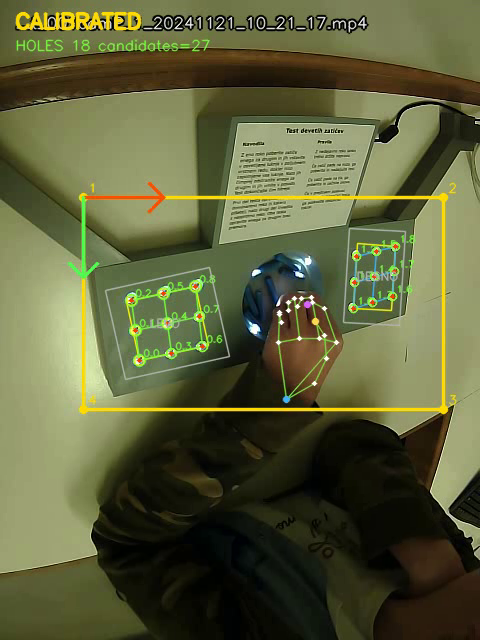
\includegraphics[width=\linewidth]{fig/article/calibrated_frame.png}\\
(a) Kalibrirana merilna površina in območja zanimanja.
\end{minipage}
\hfill
\begin{minipage}[t]{0.48\textwidth}
\centering
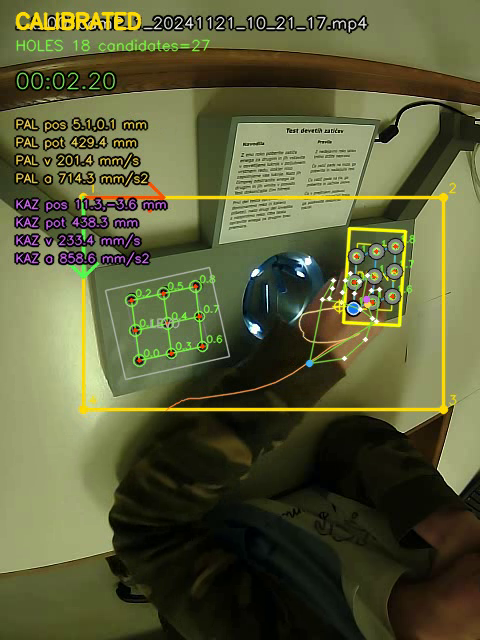
\includegraphics[width=\linewidth]{fig/article/hand_landmarks_frame.png}\\
(b) Zaznane značilke roke, palca in kazalca.
\end{minipage}
\caption{Primer obdelanega videookvirja. Kalibracija določi ploščo, mreži lukenj in lokalna območja zanimanja, MediaPipe pa poda strukturirane točke roke.}
\label{fig:frames}
\end{center}
\end{figure*}

Slika \ref{fig:frames} prikazuje delovanje kalibracije in zaznave roke na istem tipu posnetka. Kalibrirana območja omogočajo izločitev relevantnih delov slike, zato se pri nadaljnji obdelavi ne obravnava celotna slika, temveč le geometrijsko smiselna območja.

\begin{figure}[htb]
\centering
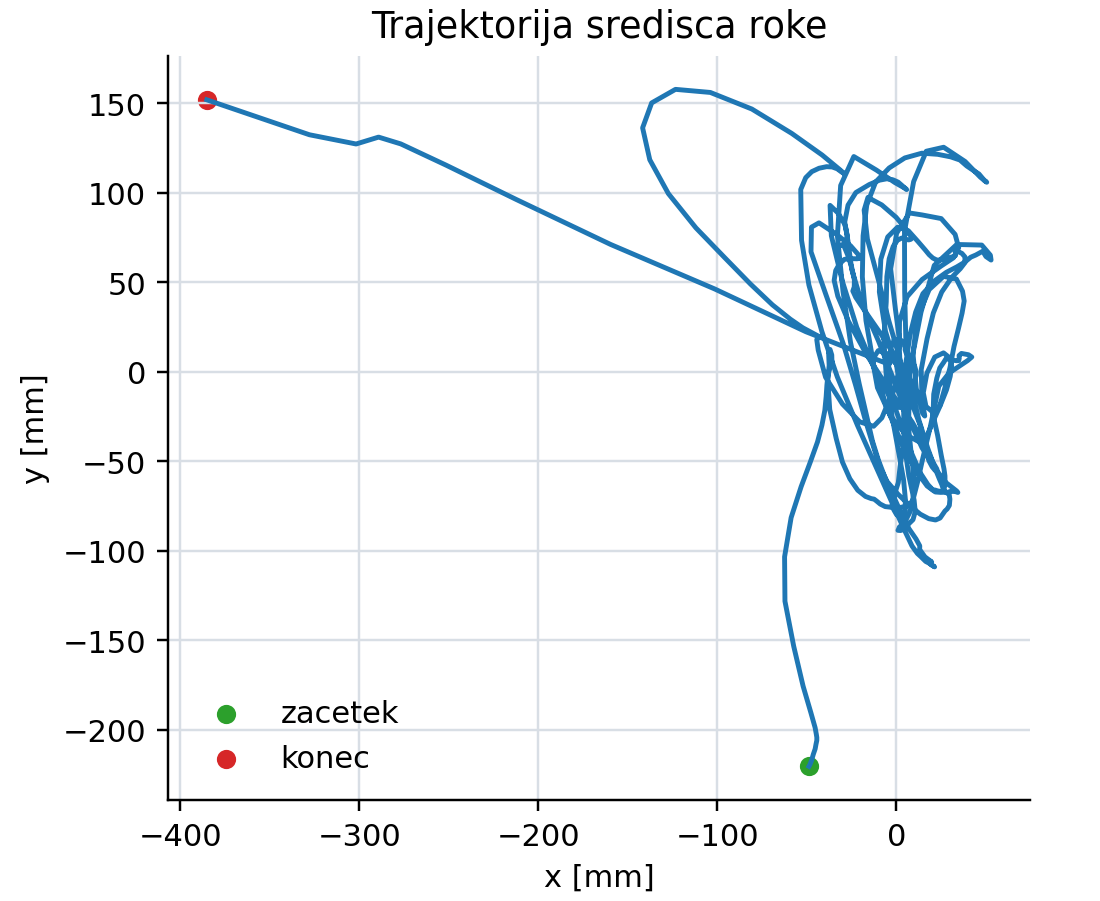
\includegraphics[width=\linewidth]{fig/article/hand_trajectory.png}
\caption{Trajektorija središča roke v koordinatnem sistemu kalibrirane plošče. Osi so podane v milimetrih.}
\label{fig:trajectory}
\end{figure}

Trajektorija na sliki \ref{fig:trajectory} kaže pretežno ponavljajoče se premike med območjem zatičev in ciljnim poljem. Ker je uporabljena ravninska preslikava, so koordinate interpretirane kot projekcija gibanja na ravnino plošče. Iz nje ni mogoče neposredno sklepati o višini roke nad ploščo.

\begin{figure}[htb]
\centering
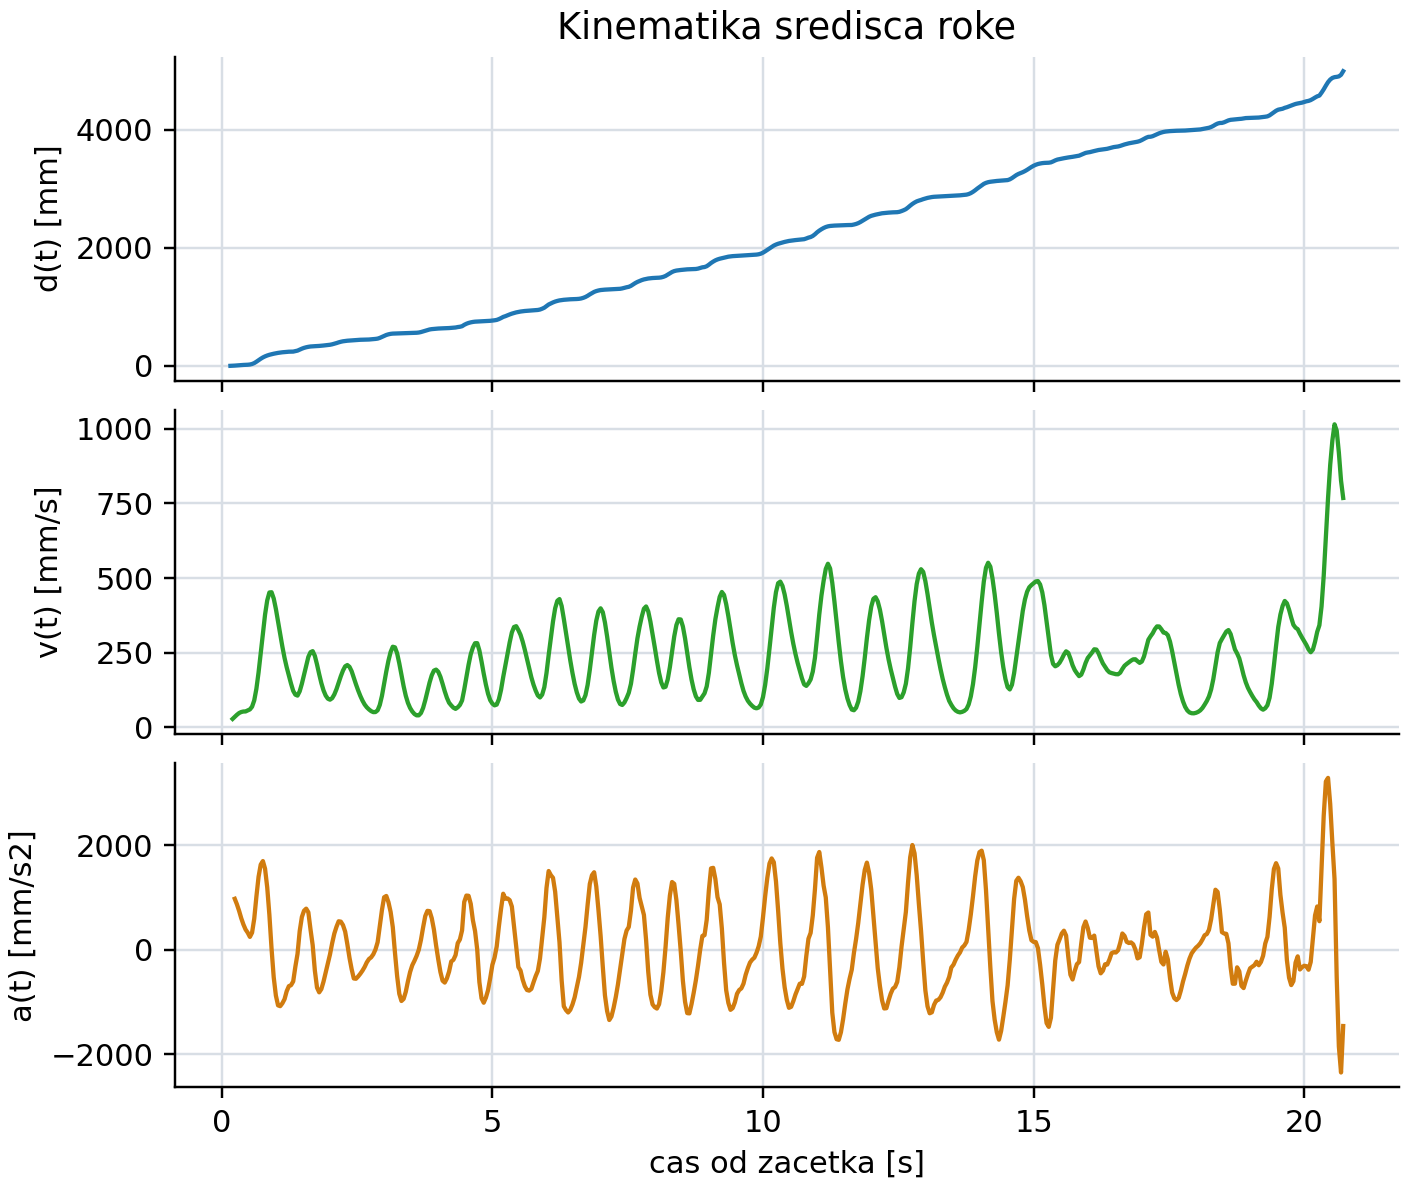
\includegraphics[width=\linewidth]{fig/article/hand_kinematics.png}
\caption{Kumulativna pot, hitrost in pospešek središča roke.}
\label{fig:handkin}
\end{figure}

Na sliki \ref{fig:handkin} so prikazani osnovni kinematični parametri središča roke. Skupna pot v ravnini je znašala približno 4,99 m, povprečna glajena hitrost 236 mm/s, največja glajena hitrost pa približno 1015 mm/s. Pospešek je izrazito nihajoč, kar je pričakovano pri diskretnem odvajanju položaja in pri gibih, ki vsebujejo hitre spremembe smeri. Zato je pospešek bolj občutljiv na šum kot pot ali hitrost.

\begin{figure}[htb]
\centering
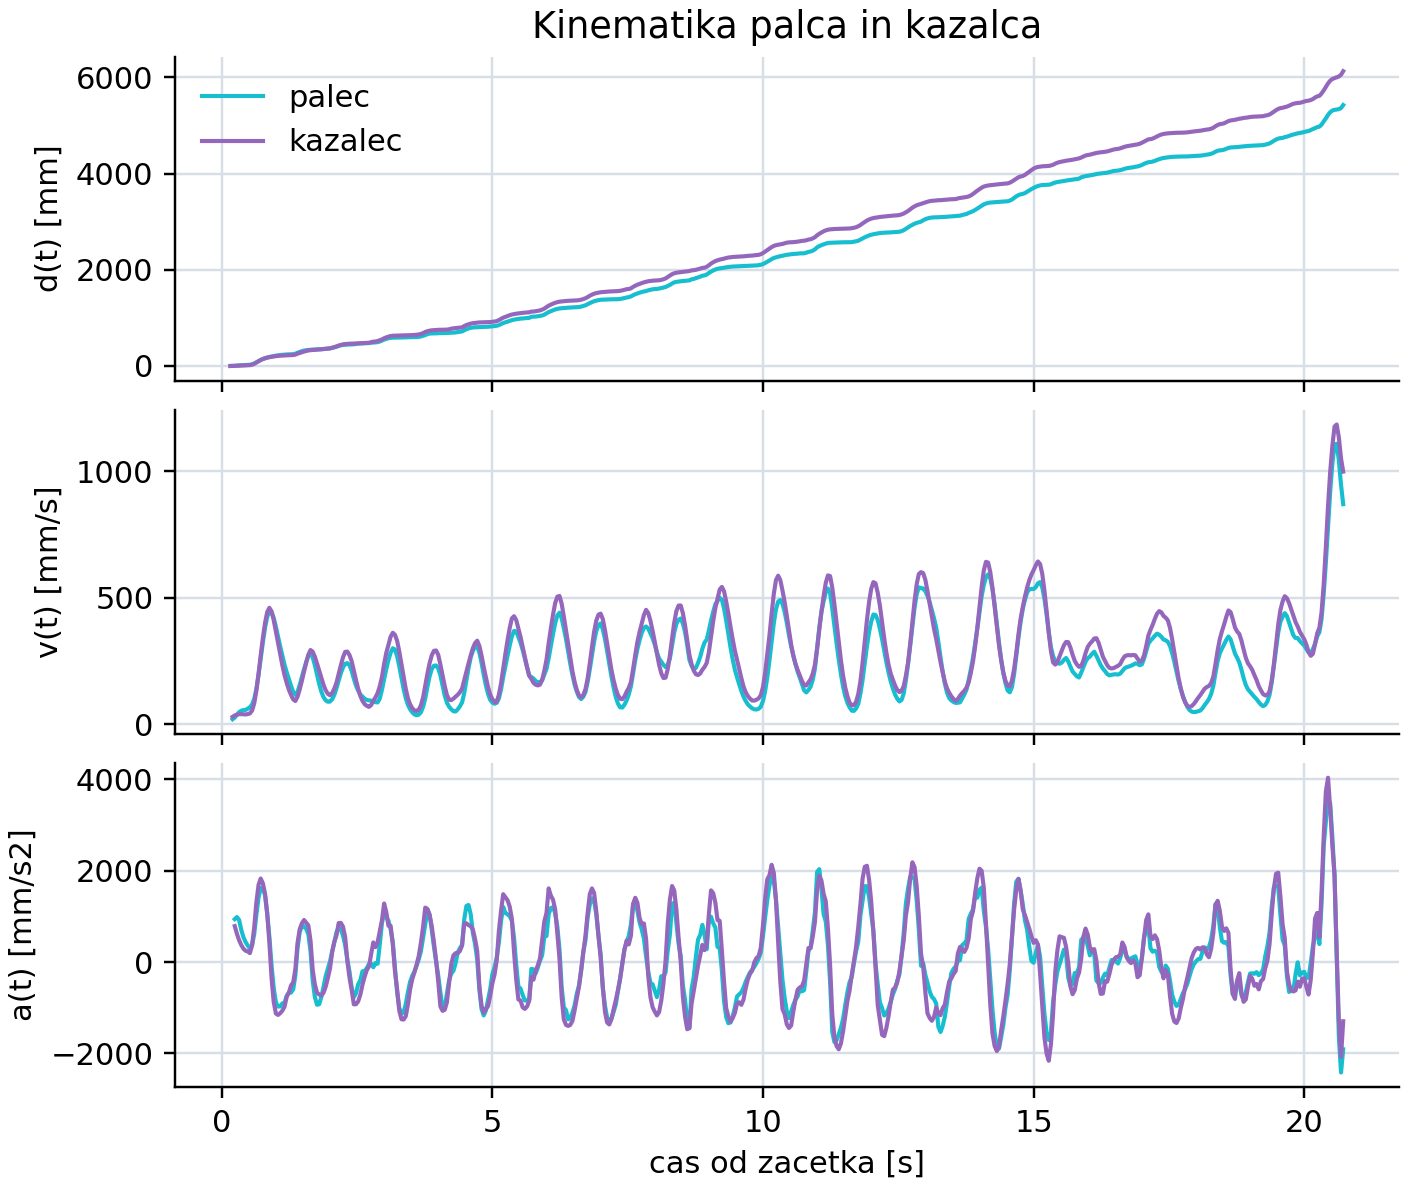
\includegraphics[width=\linewidth]{fig/article/thumb_index_kinematics.png}
\caption{Ločen izračun poti, hitrosti in pospeška za palec in kazalec.}
\label{fig:fingerkin}
\end{figure}

Slika \ref{fig:fingerkin} prikazuje dodatni podizziv: ločeno kinematiko palca in kazalca. Na izbranem posnetku je bila ocenjena pot palca približno 5,42 m, pot kazalca pa približno 6,13 m. Večja pot kazalca je smiselna, ker je konica kazalca pri prijemu pogosto bolj izpostavljena in opisuje večje lokalne premike kot središče roke.

\begin{figure}[htb]
\centering
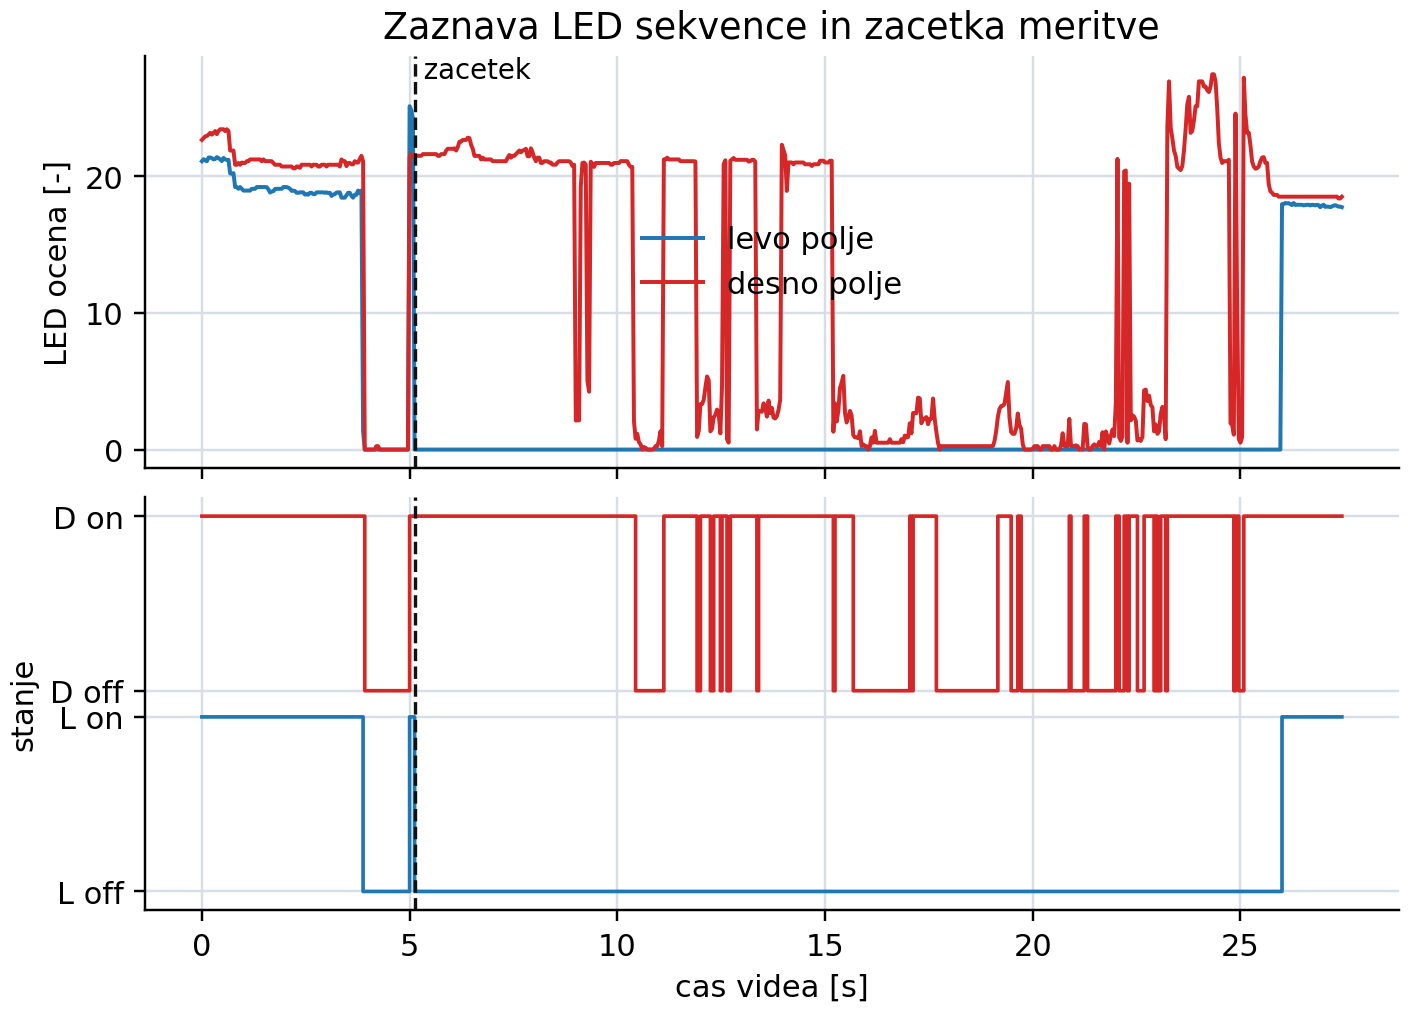
\includegraphics[width=\linewidth]{fig/article/led_sequence.png}
\caption{Zaznava LED sekvence. Vertikalna črtkana črta označuje začetek merjenja časa po stabilni prižgani ciljni strani.}
\label{fig:led}
\end{figure}

Slika \ref{fig:led} prikazuje časovni potek LED ocen. Začetek ni določen pri prvem svetlem signalu, temveč šele po zaporedju obeh prižganih polj, ugasnitve in nato stabilne ciljne strani. Tak pristop zmanjša verjetnost napačnega začetka zaradi kratkotrajnih sprememb svetlosti.

\begin{figure}[htb]
\centering
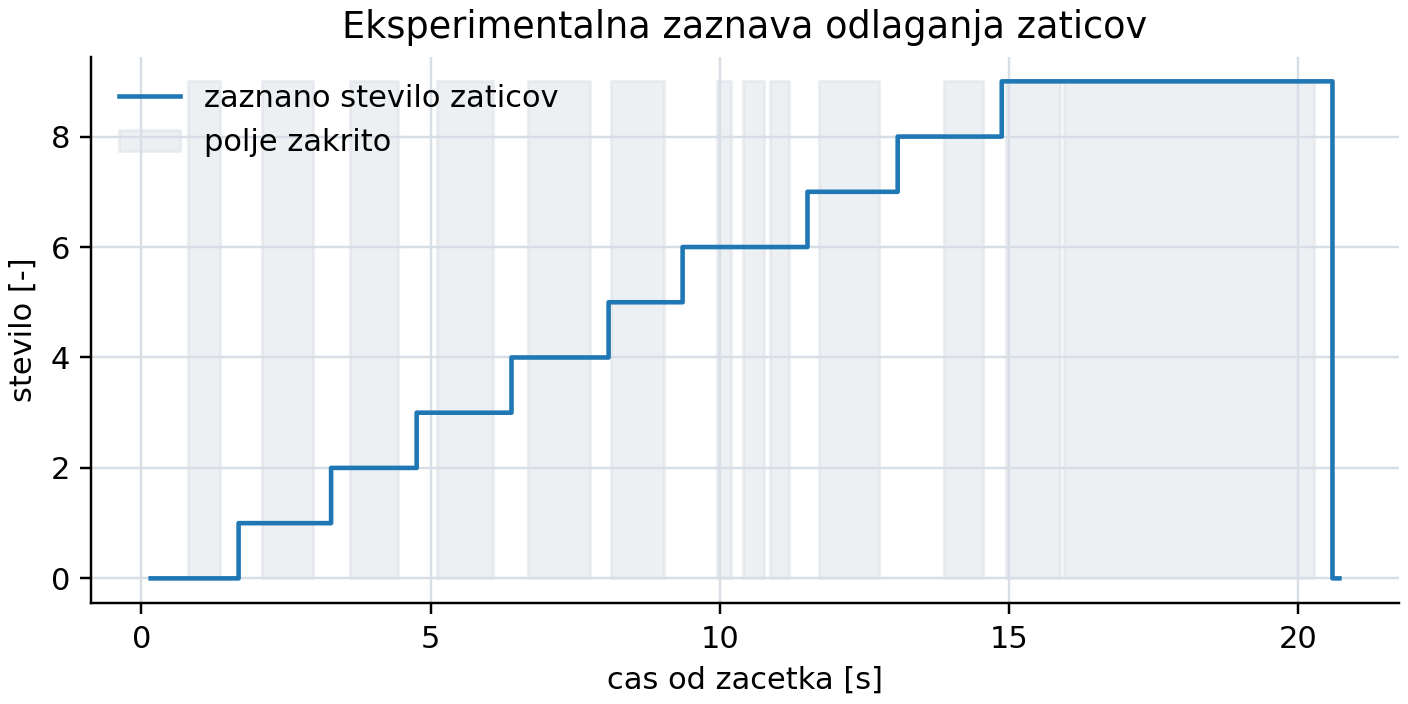
\includegraphics[width=\linewidth]{fig/article/peg_detection_experiment.png}
\caption{Eksperimentalna zaznava odloženih zatičev na ciljnem polju. Osenčeni deli označujejo okvirje, v katerih je bilo polje zakrito z roko.}
\label{fig:peg}
\end{figure}

Na sliki \ref{fig:peg} je prikazan primer eksperimentalne zaznave zatičev. Na tem posnetku je metoda sledila postopnemu naraščanju števila zaznanih zatičev in dosegla vrednost devet, vendar ta rezultat ne pomeni splošne robustnosti. Delovanje je odvisno od stabilnosti osvetlitve, vidnosti lukenj in tega, ali roka po odlaganju dovolj jasno zapusti ciljno polje.

\section{Razprava}

Največja prednost uporabe MediaPipe je strukturirana zaznava roke brez ročne segmentacije kože. Sistem dobi položaje prstov, zapestja in celotne dlani tudi v primerih, ko je ozadje kompleksno. To omogoča neposredno kinematično analizo palca in kazalca, ki bi bila z običajnimi barvnimi pragovi precej težja. Slabost takega pristopa je, da je rezultat odvisen od naučenega modela in kakovosti posnetka. Pri delnem izhodu roke iz kadra, močnih zakritjih ali nenavadnih položajih prstov se zaznava lahko izgubi.

Poseben problem je preskok zaznave na drugo roko. Če sta v kadru obe roki, lahko model v posameznem okvirju poda višjo zanesljivost za napačno roko. Zato je pomembno, da sledenje ne temelji samo na oznaki leve ali desne roke, temveč na kontinuiteti položaja, lokalnem gibanju in območju merilne plošče. Mehka omejitev območja zanimanja je pri tem kompromis: preprečuje nenadne preskoke na oddaljeno roko, hkrati pa ne prekine sledi takoj, ko roka delno zapusti območje.

Vpliv osvetlitve je dvojen. Pri LED sekvenci so svetlobne spremembe namerni signal in se pojavljajo na znanih mestih, zato je mogoče uporabiti lokalne primerjave in stroj stanj. Zaznava začetka je zato razmeroma robustna. Pri zatičih pa sprememba ni tako izrazita: zatič je majhen, njegova barva se lahko zlije z okolico, luknjo lahko zakrije senca ali prst, odsev na plošči pa lahko povzroči podobno spremembo kot dejanska prisotnost zatiča. Zato zaznava zatiča v luknji ostane manj zanesljiva in mora biti predstavljena kot eksperimentalna.

Omejitev enega pogleda kamere je, da sistem meri le projekcijo gibanja na ravnino. Hitri dvigi roke nad ploščo, spremembe višine in nagib prstov niso neposredno merljivi. Homografija dobro popravi perspektivo za točke, ki ležijo na plošči, vendar se roka in prsti gibljejo nad ploščo. Posledično so metrične koordinate približek ravninske projekcije, ne popolna tridimenzionalna rekonstrukcija.

\section{Zaključek}

Predstavljena rešitev omogoča avtomatsko analizo gibanja roke pri testu devetih zatičev iz enega videoposnetka. Glavni prispevki so kalibracija merilne površine, zaznava in sledenje roke z MediaPipe, pretvorba koordinat v realne ravninske enote ter izračun poti, hitrosti in pospeška. Poleg središča roke se ločeno analizirata palec in kazalec, kar bolje opiše gibanje prijema. Začetek merjenja časa je določen z LED sekvenco in je zato zanesljivejši od neposrednega ugibanja začetka iz položaja roke.

Nadaljnje izboljšave naj se osredotočijo na robustnejše vzdrževanje identitete izbrane roke, kombiniranje več signalov pri zaznavi odloženega zatiča, vrednotenje na večjem številu videoposnetkov in primerjavo z referenčnimi meritvami. Za natančnejšo prostorsko analizo bi bilo smiselno uporabiti dodatni pogled kamere ali globinsko informacijo, s čimer bi se zmanjšala omejitev ravninske projekcije.

\begin{thebibliography}{3}
\bibitem{mathiowetz}
V.~Mathiowetz, K.~Weber, G.~Kashman in G.~Volland, ``Adult norms for the Nine Hole Peg Test of finger dexterity,'' {\em Occupational Therapy Journal of Research}, vol.~5, no.~1, str.~24--38, 1985.

\bibitem{mediapipe}
C.~Lugaresi et al., ``MediaPipe: A framework for building perception pipelines,'' {\em arXiv preprint arXiv:1906.08172}, 2019.

\bibitem{rvgradivo}
Ž.~Špiclin, {\em Robotski vid: predavanja in laboratorijske vaje}. Fakulteta za elektrotehniko, Univerza v Ljubljani.
\end{thebibliography}

\vfill

\label{finish}

\end{document}
